\cotefile{156-4}
\scanpage{2}
\mspage{1}
\margin{\begin{tabular}{|l}\unsure{GF|CF} $\overline{\underline{\mathrm{IV}}}$\\\hline\end{tabular}}
\uline{Analysis situs} (\unsure{première mouture}).

(10 juin 1986)

1. Comme modèle ``\unsure{ensembliste} topologique de l'axiomatique d'un ``\unsure{modèle|monde} de \unsure{formes|forme} \inserted{\unsure{topologiques|topologique}}'' (ou d'une ``\uline{\unsure{contrée}}''),
considérons les notions \unsure{suivantes} \unsure{attachées} \unsure{à|:} un ``espace'' $\pm$ \unsure{ordinaire} $\deleted{\unsure{X}}\unsure{E|X}$.
On supposera ici que $\deleted{X}E$ \unsure{est} un espace topologique séparé, \unsure{ou} un espace modéré (pas néc. compact) pour une théorie \unsure{modérée} donnée.

Dans ce cas ``partie fermée'' signifie ``partie fermée \unsure{modérée}''

I) \uline{Figure} \qquad Une \uline{figure} \inserted{$F$} de $\deleted{X}E$ est une partie fermée $X$, \uline{munie} d'une
% slanted
\margin{$X$ est appelé le \uline{support} de la figure $\operatorname{supp} F$ ou $\lvert F\rvert$}
décomposition de $Y$ en \deleted{\unsure{strates}} \inserted{parties} $X_i$
\[
\{X_{\unsure{i}}\}\in\unsure{\mathcal{P}|D}(Y) \qquad X=\bigcup X_i
\]
appelées les \uline{strates fermées}. On fait les hypothèses

a) Les $X_i$ fermés \inserted{non vides et loc. compacts (loc. \unsure{cpt|cpt.} est \unsure{autom.} si $\deleted{X}E$ l'est, par ex. \unsure{Esp. mod.})} (pas néc. compacts \unsure{\}} \deleted{\illegible{1}} \unsure{ils le s\textsuperscript{t}} si $X$ l'est\unsure{)}

b) La famille des $X_i$ est loc. finie
\inserted{(donc par a) b) \unsure{d'où|d} $\Rightarrow$ réunion \unsure{de|des} str.~f. est fermée\unsure{)}}
\margin{NB on pose $i\leq j\iff X_i\unsure{\subset|\in}X_j$ \quad $i<j\iff X_i\unsure{\subsetneqq|\nsubseteq}X_j$}

c) Si \deleted{\unsure{$X_i=$}} \deleted{\unsure{$\partial X_i=$}} $X_i\subset X_j$, $X_i\ne X_j$, (i.e. $i<j$) alors $X_i$ \uline{rare} dans $X_j$

d) Posant $\partial X_i=\deleted{\unsure{\bigcup_{X_j\subsetneq X_i}X_j}}\bigcup_{j<i}X_j$ (donc $\partial X_i$
\scanpage{3}
\mspage{2}
est fermé rare \unsure{en|dans} $X_i$, par a) b) c)) \deleted{\unsure{est}} $\operatorname{int}(X_i)=X_i\setminus\partial X_i$, lequel est donc un ouvert \inserted{rel.} dense de $X_i$, et non vide puisque $X_i$ l'est) est \deleted{\unsure{une}} 1\textsuperscript{o}) \uuline{variété} 2\textsuperscript{o}) \uline{connexe}. (NB dans le cas $E$ modéré, on prend ``variété'' au sens modéré, certes.)
% slanted
\margin{e) Si $\deleted{X_i\unsure{<|\subset}X_j}\inserted{i<j}$ alors $\dim\unsure{\text{l'int}|\operatorname{int}|\operatorname{ind}}(X_i)<\dim\unsure{\operatorname{int}|\operatorname{ind}}(X_j)$, pour éviter des \unsure{phénomènes} de \unsure{sauvagerie}}
% slanted; orient the marginal drawing as on the sheet
\figure{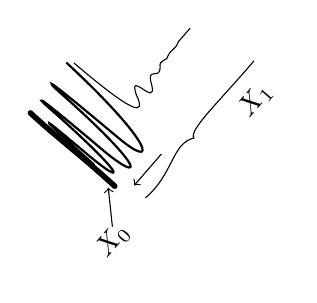
\begin{tikzpicture}[x=.85cm,y=.85cm]
\begin{scope}[rotate=49]
\draw[line width=2pt,line cap=round] (0,0) .. controls (.02,.7) and (-.02,1.15) .. (0,1.67);
\draw[line width=.8pt] (.04,.44) .. controls (.055,1.57) and (.075,1.67) .. (.09,.68)
 .. controls (.10,-.20) and (.23,-.04) .. (.24,1.60)
 .. controls (.26,1.87) and (.28,1.30) .. (.29,.49)
 .. controls (.31,-.34) and (.51,-.17) .. (.52,1.64)
 .. controls (.54,1.88) and (.56,1.58) .. (.58,.46)
 .. controls (.59,-.35) and (.86,-.05) .. (.92,1.76);
\draw (.99,1.67) .. controls (1.00,.48) and (1.10,.33) .. (1.24,.65)
 .. controls (1.45,1.01) and (1.29,.29) .. (1.50,.57)
 .. controls (1.67,.84) and (1.62,.53) .. (1.78,.65)
 .. controls (1.87,.76) and (1.93,.62) .. (2.00,.68)
 .. controls (2.11,.71) and (2.16,.65) .. (2.25,.70) -- (2.52,.70);
\draw[<-] (.20,-.21) -- (.82,-.21);
\draw (.17,-.46) .. controls (.72,-.54) and (1.05,-.22) .. (1.32,-.42)
 .. controls (1.34,-.28) and (2.00,-.35) .. (2.78,-.34);
\draw[->] (-.48,-.37) -- (-.08,.06);
\node[rotate=49] at (-.63,-.51) {$X_0$};
\node[rotate=49] at (2.35,-.74) {$X_1$};
\end{scope}
\end{tikzpicture}}

\deleted{\unsure{e}}f) $X_i\cap X_j$ est réunion \unsure{de|des} $X_k$.

Donc une figure \inserted{$F$} peut s'identifier à l'ens de ses strates, qui est un ens de parties fermées \unsure{de|sur|en} $X$
\[
\underset{\substack{\shortparallel\\\{X_i\}}}{F}\subset\unsure{\mathcal{P}|D}_f(x)
\qquad \text{i.e.}\qquad F\in\mathcal{P}(\mathcal{P}_f(X))
\]
($X$ se \unsure{réconstitue} comme $\bigcup X_i$), satisfaisant certaines conditions \inserted{(qu'on vient d'expliciter, a) à d))}. On a donc l'ens des figures, \deleted{qui} soit $\mathcal{F}$, qui est donc un ens. de parties de $\mathcal{P}_f(x)$
\[
\mathcal{F}\subset\mathcal{P}(\mathcal{P}_f)\qquad\text{i.e.}\qquad
\mathcal{F}\in\mathcal{P}(\mathcal{P}(\mathcal{P}_f(X\unsure{)))|))}
\]

À chaque $F\in\mathcal{F}$ est associé \uline{l'ens ordonné} $\Sigma_F$ de ses strates. L'ens somme
\diagram{\begin{tikzcd}[ampersand replacement=\&,column sep=small,row sep=small]
\Sigma \arrow[d,"{\rule{16mm}{.25pt}}"'] \& {}=\displaystyle\coprod_{F\in\mathcal{F}}\Sigma_F\\
\mathcal{F} \&
\end{tikzcd}}
{\reversemarginpar\margin{les fibres sont les $\Sigma_F$}}
\margin{\uline{NB} Dans le cas d'espèce, on \unsure{à|a} $\Sigma_F\unsure{\equiv|\simeq}F$, \deleted{\unsure{mais l'ai|mais j'ai} \illegible{1} \unsure{déjà|dit}.}}
peut aussi s'identifier à l'ens des couples $(F,X_i)$, \deleted{\unsure{$F$ e}} où $F$ est une figure et $X_i$ est une strate de $F$ i.e. $X_i\in F$.
\scanpage{4}
\mspage{3}
Si $F,F'$ sont deux figures, on dit que $F'$ est une \uline{sous-figure} de $F$, si \unsure{toute|tout} strate de $F'$ est une strate de $F$, i.e. $F'\subset F$. Donc \deleted{le support} on aura \deleted{\unsure{$\sigma(F)$}} \unsure{d|et} $\lvert F'\rvert\subset\lvert F\rvert$

\uline{NB} Si $X_i\in F'$, et $Y_j\in F$ est tel que $Y_j\subset X_i$, alors $Y_j\in F'$

\deleted{En effet, soit $y\in\deleted{\unsure{Y_j}}\operatorname{int}(Y_j)$, alors}

\deleted{La relation}

On écrit $F'\leq F$ pour cette relation, qui est une relation d'ordre dans $\mathcal{F}$.

L'ens des sous-figures de $F$ est en corr. 1-1 avec l'ens des parties \inserted{$\unsure{\Phi|\varphi}$ ($=\Sigma_{F'}$)} de \deleted{\unsure{$F$|$\mathcal{F}$}} \inserted{$\Sigma_F$, (ens des strates)} qui ont la \unsure{propriét.|propriété} que \inserted{$i,j\in\Sigma_F$,} $i\in\deleted{\unsure{\Sigma|B}}\Phi$, $j\leq i\Rightarrow j\in\Phi$
(\deleted{idéaux} \inserted{``\unsure{fermés|les parties|fermées}''} \deleted{fermés} de l'ens \deleted{\unsure{ens}} ordonné, pour la top. \inserted{sur $\Sigma_F=\Sigma$} \unsure{ayant} comme base \deleted{de fermés} \deleted{d'ouverts \unsure{/} les} \inserted{d'ouverts les} $\Sigma_{\deleted{\unsure{>}}\unsure{\geq|\leq}i}$).

\deleted{\unsure{Ainsi|$F'\leq F$}, on a une relation d'ordre sur}
% slanted
\margin{\uline{11.6.} Je dirai \unsure{plus tôt|plutôt} ``\uline{\unsure{multistrate}}''}

\uline{Figure élémentaire} : qui a une strate maximale i.e. $\Sigma_F$ a un plus grand élément. Soit \tikz[baseline=(el.base)]{\node[inner sep=1pt] (el) {$\mathcal{F}_{\text{él}}$};\draw (el.center) ellipse [x radius=1.05em,y radius=.78em];} l'ens des figures élémentaires. \deleted{Alors} Pour tte figure $F$, les sous-figures élémentaires sont en corr 1-1 avec les
\scanpage{5}
\mspage{4}
strates de $F$. \deleted{Donc on peut \unsure{ide|idé}}
\[
\begin{aligned}
 F &\quad \text{figure}\\
 \Sigma_F &\quad \text{ens de ses strates}\\
 \Sigma'_F &\quad \text{ens des sous-figures élémentaires.}
\end{aligned}
\]
On \unsure{:|a|=}
\diagram{\begin{tikzcd}[ampersand replacement=\&,column sep=small,row sep=.35em]
\Sigma'_F \& {}\simeq\Sigma_F\\
{\unsure{\rotatebox{-90}{$\subset$}|\cap|\rotatebox{-90}{$\in$}}} \&\\
\mathcal{F}_{\text{él}} \&
\end{tikzcd}}
$F$ est connu quand on \unsure{connait|connaît} $\Sigma'_F\unsure{\subset|\in}\mathcal{F}_{\text{él}}$ \unsure{Car|car} $F$ est l'ens des strates \unsure{des|de} $F'\in\Sigma'_F$.

Mais la relation d'inclusion entre figures \unsure{s'interprete|s'interprète} comme relation d'inclusion entre \unsure{partie|parties} de $\mathcal{F}_{\unsure{\text{él}|\text{el}}}$.

\deleted{Deux \unsure{f}}

Considérons la relation d'inclusion \inserted{$\leq$} entre figures élémentaires. \deleted{\unsure{A}}Alors, $\mathcal{F}_{\text{él}}$ est un ens ordonné. \deleted{Deux} \inserted{Si} \deleted{figures sont dites} \inserted{$F$ est une figure,} $\Sigma'_F$ est une partie fermée de l'ens ordonné $\mathcal{F}_{\text{él}}$. L'\unsure{inclussion|inclusion} entre figures est l'inclusion entre ces parties fermées.
\scanpage{6}
\mspage{5}
\deleted{Pour qu'une partie $\unsure{\Phi|\varphi}$ de $\mathcal{F}_{\text{él}}$ soit de la forme $\Sigma_F$, il \unsure{f|f.} et s.}

\deleted{a) Que $\Phi$ soit une partie fermée de $\mathcal{F}_{\text{él}}$}

\deleted{b) Que la \deleted{\illegible{1}} \inserted{famille} des $\lvert\varphi\rvert$,}

\deleted{Deux figures \inserted{$F,\deleted{\unsure{X}}F'$} sont dites}

\deleted{Considérons deux figures $F,F'$, et les conditions}
\[
\deleted{\lvert F\rvert\cap\lvert F'\rvert}\,.
\]

Soit $F$ une figure, une partie \deleted{\unsure{fermée}} $A$ de $\lvert F\rvert=\operatorname{supp} F$ est dite saturée (pour $F$), ou $F$-saturée, si elle est saturée pour la relation d'équ. définie par les $\deleted{\unsure{X_2|X_i|X_j}}\overset{\substack{\inserted{\text{strate ``ouverte''}}\\[-.45ex]\raisebox{-.5ex}{\rule{.4pt}{.6ex}}\rule{4.4em}{.4pt}\raisebox{-.5ex}{\rule{.4pt}{.6ex}}}}{\operatorname{int}(\unsure{X'|X_i})}$ (où $(X_i)$ est l'ens des strates). Si $A$ est \unsure{fermé|fermée}, cela signifie que \unsure{$A$ est|$A$} réunion de strates (fermées)
% slanted
\margin{Relation de saturation stable pour $\cap,\ \cup,\ \unsure{\complement_{\lvert F\rvert}|C_{\lvert F\rvert}}\unsure{(}$ \unsure{$-$}. Si $F'$ est une sous-figure de $F$, et \unsure{$\exists$|$\mathcal{F}$|$\forall$} : $A\subset\lvert F'\rvert$, alors \unsure{$A$} est $F'$-saturée ssi $A$ est \unsure{$\exists$|$\mathcal{F}$} $F$-saturée (car $\lvert F'\rvert$ est \unsure{$\lvert F\rvert$|$F$} saturé \unsure{lui-$=$|lui-m\textsuperscript{me}})}

\unsure{Soit|Soient} $F,F'$ deux figures.

Considérons les conditions

\deleted{a) $\lvert F\rvert\cap\lvert F'\rvert$ est $F$-saturé et $F'$-saturé}

a) $\forall X\in\Sigma_F$, $X'\in\Sigma_{F'}$, $X\cap X'$ est \deleted{\unsure{$F$-satu}} $F_X$-saturé \deleted{\unsure{de} \unsure{$F_X$-Sat}} et \deleted{\unsure{$F_{X'}$}-}$\unsure{F|F'|B}$-saturé
\scanpage{7}
\mspage{6}
\deleted{c) $\exists$ \unsure{Sous-figure|sous-figure} $F''$, \unsure{telle} que}

\deleted{1°) $F''$ sous-figure de $F$, et de $F'$}

\deleted{2°) \unsure{Toute} $\unsure{(F\smallsetminus F'')|(\lvert F\rvert\smallsetminus F'')}\cap(\lvert F'\rvert\smallsetminus F''$}

\deleted{Si \unsure{le|la} $U$ strate ouverte de $F$, $U'$ \unsure{strate}}

b) Si $U_i$ est une \deleted{cellule}\inserted{strate} ouverte de $F$. $U'_j$ strate ouverte de $F'$, alors on a $U_i\cap U'_j=\varnothing$ \uline{ou} $U_i=U'_j$.

Ces conditions sont \unsure{équivalentes|equivalentes}

\deleted{car $b\Rightarrow a$ trivial (puisque $\lvert F\rvert=\bigcup X_i$, $\lvert F'\rvert=\bigcup X'_j$)}

\deleted{$\unsure{a\Rightarrow b|a\Rightarrow a}$}

b) $\Rightarrow$ a) trivial, prouvons a) $\Rightarrow$ b) \deleted{Si} Supposons que $U_i\cap U'_j\ne\varnothing$, \deleted{$U_i\ne U'_j$ alors} \inserted{prouvons $U_i=U'_j$}

\deleted{$X_i\ne X'_j$ Considérons $X_i\cap X'_j$ $(\unsure{+|\ne}\varnothing$,}

\unsure{''} Soit \deleted{\illegible{1}}\inserted{$x\in$} \deleted{\unsure{$U_i\cap U'_j$}}, Considérons $X_i\cap X'_j$, \deleted{et le} Comme $X_i\cap X'_j$ est \inserted{fermé} $F_{X_i}$-saturé, \deleted{\unsure{pour}}\inserted{et} \deleted{et que $\unsure{x\in}X_i\cap X'_j$,} \inserted{contient $x\in U_i$, on} on a $X_i\subset X_i\cap\unsure{X''_j|X'_j}$,
\deleted{\unsure{donc on}} i.e. $X_i\subset X'_j$. De $=$ $X'_j\subset X_i$ Donc on a $X_i=X'_j$. On ne peut en conclure encore directement $\deleted{X_i}U_i=U'_j$, \deleted{car il} \unsure{i.e.|'' n.} $\partial X_i=\partial X'_j$. Mais
On \deleted{le} prouve \inserted{a) $\Rightarrow$ b)} par récurrence sur \deleted{dim de} $\operatorname{Sup}(\dim\deleted{X}F,\dim F')$ (on est ramené au cas des figures $F_{X_i}$, $F'_{X'_j}$, i.e. au cas de la dim \unsure{finie|facile|$+$ basse}\ldots)
\scanpage{8}
\mspage{7}
On dit que $F,F'$ sont \uline{compatibles} si les conditions en question sont \unsure{satisfaites}.

Pour \unsure{ceci|cela}, il \unsure{f|f.} et \unsure{s.|s} que pour \unsure{toute|tous} $F_0\in\Sigma'_F$, $F'_0\in\Sigma'_{F'}$, $F_0$ et $F''_0$ soient compatibles.

Donc, dans l'ens \inserted{ordonné $\mathcal{F}_{\text{él}}$} des figures élémentaires, on introduit une relation (\unsure{symetrique|symétrique}, \unsure{reflexive|réflexive})
\[
\begin{aligned}
&\mathcal{R}\subset\mathcal{F}_{\text{él}}\times\mathcal{F}_{\text{él}}&&\deleted{\{\unsure{F,F'|F_0,F'_0}\}}\quad \text{$F_0$ comp. avec $F'_0$}\\
\text{ou encore}\quad&\mathcal{S}\in\mathcal{P}_2(\mathcal{F}_{\text{él}})&&\deleted{\text{\unsure{ou|cou}}}\quad\text{\uline{paires compatibles}}
\end{aligned}
\]
\uline{NB} Si \deleted{\unsure{$X$|$2$}} $F_0\to F'_0$ sont des fig. él. telles que $F_0\le F'_0$, alors elles sont compatibles. Mieux, si $F'_0,F''_0\le F$, alors $F_0$ et $F'_0$ sont compatibles entre elles

\uline{Configuration} Ens de figures deux \unsure{:|à} deux compatibles. Configuration élémentaire : ens des figures élémentaires deux \unsure{2|à} deux compatibles.
\scanpage{9}
\mspage{8}
Soit $F$ une figure, \deleted{$\unsure{\Sigma'|\Sigma}$}
\[
\Sigma'_F=\unsure{\Phi|\varphi}\subset\mathcal{F}_{\text{él}}
\]
la partie de $\mathcal{F}_{\text{él}}$ associée. \deleted{\unsure{S|A}}Alors on a les conditions

a) $\Phi$ est fermée dans l'ens \unsure{ordonné|ordonn} $\mathcal{F}_{\text{él}}$

b) Si \deleted{$\unsure{F_0,F'_0|F_0,F'_2}\ \unsure{\Rightarrow|\ne|\in}$} $F_1,F_2\in\Phi$, \inserted{$F_1\ne F_2$} alors $F_1,F_2$ sont compatibles, i.e. $\Phi$ est une \uline{configuration}

c) $\Phi$ est ``loc. \unsure{finie|fini}'' en un sens convenable.

\unsure{Donc} si on ne veut exclure \unsure{les|le} cas des figures infinies, il faut aussi \unsure{considérer} dans $\mathcal{F}_{\unsure{\text{el}|\text{él}}}$ \unsure{lá|la|là} donnée des parties loc. finies (i.e. dont la famille des \unsure{supports|support} dans $X$ est loc finie) qui \unsure{forment|forme} un antifiltre dans $\mathcal{F}_{\text{el}}$.

\unsure{Inversement}, \unsure{tout|toute} $\Phi$ satisfaisant a) b) c) provient d'une figure et d'une seule.
